\documentclass[1p]{elsarticle_modified}
%\bibliographystyle{elsarticle-num}

%\usepackage[colorlinks]{hyperref}
%\usepackage{abbrmath_seonhwa} %\Abb, \Ascr, \Acal ,\Abf, \Afrak
\usepackage{amsfonts}
\usepackage{amssymb}
\usepackage{amsmath}
\usepackage{amsthm}
\usepackage{scalefnt}
\usepackage{amsbsy}
\usepackage{kotex}
\usepackage{caption}
\usepackage{subfig}
\usepackage{color}
\usepackage{graphicx}
\usepackage{xcolor} %% white, black, red, green, blue, cyan, magenta, yellow
\usepackage{float}
\usepackage{setspace}
\usepackage{hyperref}

\usepackage{tikz}
\usetikzlibrary{arrows}

\usepackage{multirow}
\usepackage{array} % fixed length table
\usepackage{hhline}

%%%%%%%%%%%%%%%%%%%%%
\makeatletter
\renewcommand*\env@matrix[1][\arraystretch]{%
	\edef\arraystretch{#1}%
	\hskip -\arraycolsep
	\let\@ifnextchar\new@ifnextchar
	\array{*\c@MaxMatrixCols c}}
\makeatother %https://tex.stackexchange.com/questions/14071/how-can-i-increase-the-line-spacing-in-a-matrix
%%%%%%%%%%%%%%%

\usepackage[normalem]{ulem}

\newcommand{\msout}[1]{\ifmmode\text{\sout{\ensuremath{#1}}}\else\sout{#1}\fi}
%SOURCE: \msout is \stkout macro in https://tex.stackexchange.com/questions/20609/strikeout-in-math-mode

\newcommand{\cancel}[1]{
	\ifmmode
	{\color{red}\msout{#1}}
	\else
	{\color{red}\sout{#1}}
	\fi
}

\newcommand{\add}[1]{
	{\color{blue}\uwave{#1}}
}

\newcommand{\replace}[2]{
	\ifmmode
	{\color{red}\msout{#1}}{\color{blue}\uwave{#2}}
	\else
	{\color{red}\sout{#1}}{\color{blue}\uwave{#2}}
	\fi
}

\newcommand{\Sol}{\mathcal{S}} %segment
\newcommand{\D}{D} %diagram
\newcommand{\A}{\mathcal{A}} %arc


%%%%%%%%%%%%%%%%%%%%%%%%%%%%%5 test

\def\sl{\operatorname{\textup{SL}}(2,\Cbb)}
\def\psl{\operatorname{\textup{PSL}}(2,\Cbb)}
\def\quan{\mkern 1mu \triangleright \mkern 1mu}

\theoremstyle{definition}
\newtheorem{thm}{Theorem}[section]
\newtheorem{prop}[thm]{Proposition}
\newtheorem{lem}[thm]{Lemma}
\newtheorem{ques}[thm]{Question}
\newtheorem{cor}[thm]{Corollary}
\newtheorem{defn}[thm]{Definition}
\newtheorem{exam}[thm]{Example}
\newtheorem{rmk}[thm]{Remark}
\newtheorem{alg}[thm]{Algorithm}

\newcommand{\I}{\sqrt{-1}}
\begin{document}

%\begin{frontmatter}
%
%\title{Boundary parabolic representations of knots up to 8 crossings}
%
%%% Group authors per affiliation:
%\author{Yunhi Cho} 
%\address{Department of Mathematics, University of Seoul, Seoul, Korea}
%\ead{yhcho@uos.ac.kr}
%
%
%\author{Seonhwa Kim} %\fnref{s_kim}}
%\address{Center for Geometry and Physics, Institute for Basic Science, Pohang, 37673, Korea}
%\ead{ryeona17@ibs.re.kr}
%
%\author{Hyuk Kim}
%\address{Department of Mathematical Sciences, Seoul National University, Seoul 08826, Korea}
%\ead{hyukkim@snu.ac.kr}
%
%\author{Seokbeom Yoon}
%\address{Department of Mathematical Sciences, Seoul National University, Seoul, 08826,  Korea}
%\ead{sbyoon15@snu.ac.kr}
%
%\begin{abstract}
%We find all boundary parabolic representation of knots up to 8 crossings.
%
%\end{abstract}
%\begin{keyword}
%    \MSC[2010] 57M25 
%\end{keyword}
%
%\end{frontmatter}

%\linenumbers
%\tableofcontents
%
\newcommand\colored[1]{\textcolor{white}{\rule[-0.35ex]{0.8em}{1.4ex}}\kern-0.8em\color{red} #1}%
%\newcommand\colored[1]{\textcolor{white}{ #1}\kern-2.17ex	\textcolor{white}{ #1}\kern-1.81ex	\textcolor{white}{ #1}\kern-2.15ex\color{red}#1	}

{\Large $\underline{12n_{0006}~(K12n_{0006})}$}

\setlength{\tabcolsep}{10pt}
\renewcommand{\arraystretch}{1.6}
\vspace{1cm}\begin{tabular}{m{100pt}>{\centering\arraybackslash}m{274pt}}
\multirow{5}{120pt}{
	\centering
	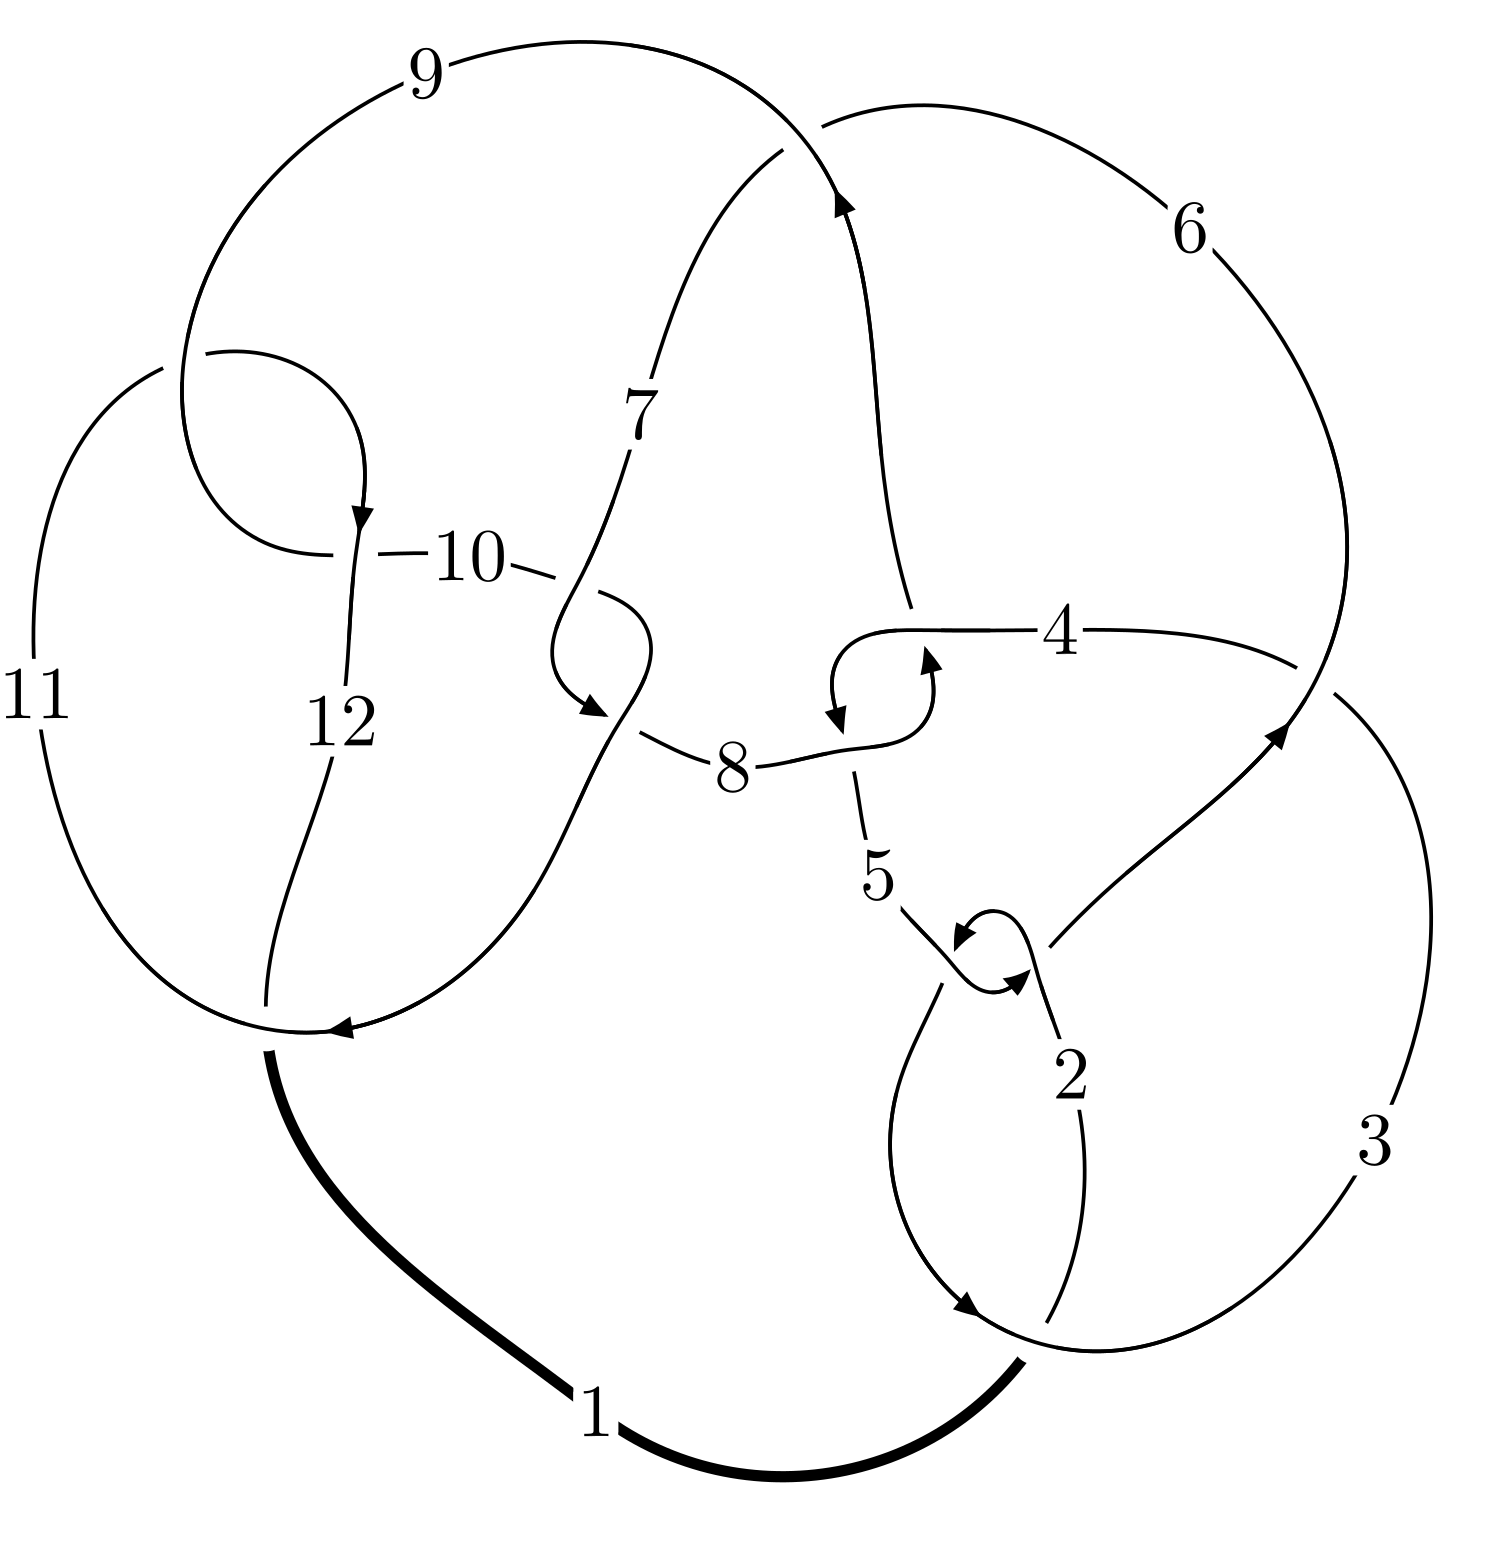
\includegraphics[width=112pt]{../../../GIT/diagram.site/Diagrams/png/2095_12n_0006.png}\\
\ \ \ A knot diagram\footnotemark}&
\allowdisplaybreaks
\textbf{Linearized knot diagam} \\
\cline{2-2}
 &
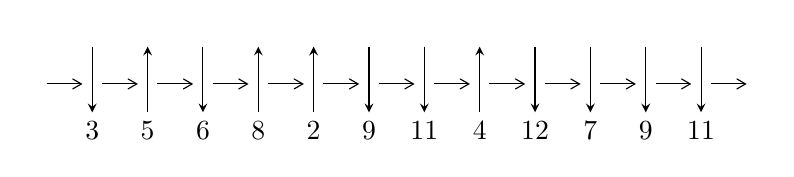
\begin{tikzpicture}[x=20pt, y=17pt]
	% nodes
	\node (C0) at (0, 0) {};
	\node (C1) at (1, 0) {};
	\node (C1U) at (1, +1) {};
	\node (C1D) at (1, -1) {3};

	\node (C2) at (2, 0) {};
	\node (C2U) at (2, +1) {};
	\node (C2D) at (2, -1) {5};

	\node (C3) at (3, 0) {};
	\node (C3U) at (3, +1) {};
	\node (C3D) at (3, -1) {6};

	\node (C4) at (4, 0) {};
	\node (C4U) at (4, +1) {};
	\node (C4D) at (4, -1) {8};

	\node (C5) at (5, 0) {};
	\node (C5U) at (5, +1) {};
	\node (C5D) at (5, -1) {2};

	\node (C6) at (6, 0) {};
	\node (C6U) at (6, +1) {};
	\node (C6D) at (6, -1) {9};

	\node (C7) at (7, 0) {};
	\node (C7U) at (7, +1) {};
	\node (C7D) at (7, -1) {11};

	\node (C8) at (8, 0) {};
	\node (C8U) at (8, +1) {};
	\node (C8D) at (8, -1) {4};

	\node (C9) at (9, 0) {};
	\node (C9U) at (9, +1) {};
	\node (C9D) at (9, -1) {12};

	\node (C10) at (10, 0) {};
	\node (C10U) at (10, +1) {};
	\node (C10D) at (10, -1) {7};

	\node (C11) at (11, 0) {};
	\node (C11U) at (11, +1) {};
	\node (C11D) at (11, -1) {9};

	\node (C12) at (12, 0) {};
	\node (C12U) at (12, +1) {};
	\node (C12D) at (12, -1) {11};
	\node (C13) at (13, 0) {};

	% arrows
	\draw[->,>={angle 60}]
	(C0) edge (C1) (C1) edge (C2) (C2) edge (C3) (C3) edge (C4) (C4) edge (C5) (C5) edge (C6) (C6) edge (C7) (C7) edge (C8) (C8) edge (C9) (C9) edge (C10) (C10) edge (C11) (C11) edge (C12) (C12) edge (C13) ;	\draw[->,>=stealth]
	(C1U) edge (C1D) (C2D) edge (C2U) (C3U) edge (C3D) (C4D) edge (C4U) (C5D) edge (C5U) (C6U) edge (C6D) (C7U) edge (C7D) (C8D) edge (C8U) (C9U) edge (C9D) (C10U) edge (C10D) (C11U) edge (C11D) (C12U) edge (C12D) ;
	\end{tikzpicture} \\
\hhline{~~} \\& 
\textbf{Solving Sequence} \\ \cline{2-2} 
 &
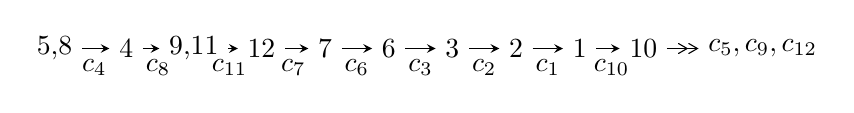
\begin{tikzpicture}[x=23pt, y=7pt]
	% node
	\node (A0) at (-1/8, 0) {5,8};
	\node (A1) at (1, 0) {4};
	\node (A2) at (33/16, 0) {9,11};
	\node (A3) at (25/8, 0) {12};
	\node (A4) at (33/8, 0) {7};
	\node (A5) at (41/8, 0) {6};
	\node (A6) at (49/8, 0) {3};
	\node (A7) at (57/8, 0) {2};
	\node (A8) at (65/8, 0) {1};
	\node (A9) at (73/8, 0) {10};
	\node (C1) at (1/2, -1) {$c_{4}$};
	\node (C2) at (3/2, -1) {$c_{8}$};
	\node (C3) at (21/8, -1) {$c_{11}$};
	\node (C4) at (29/8, -1) {$c_{7}$};
	\node (C5) at (37/8, -1) {$c_{6}$};
	\node (C6) at (45/8, -1) {$c_{3}$};
	\node (C7) at (53/8, -1) {$c_{2}$};
	\node (C8) at (61/8, -1) {$c_{1}$};
	\node (C9) at (69/8, -1) {$c_{10}$};
	\node (A10) at (11, 0) {$c_{5},c_{9},c_{12}$};

	% edge
	\draw[->,>=stealth]	
	(A0) edge (A1) (A1) edge (A2) (A2) edge (A3) (A3) edge (A4) (A4) edge (A5) (A5) edge (A6) (A6) edge (A7) (A7) edge (A8) (A8) edge (A9) ;
	\draw[->>,>={angle 60}]	
	(A9) edge (A10);
\end{tikzpicture} \\ 

\end{tabular} \\

\footnotetext{
The image of knot diagram is generated by the software ``\textbf{Draw programme}" developed by Andrew Bartholomew(\url{http://www.layer8.co.uk/maths/draw/index.htm\#Running-draw}), where we modified some parts for our purpose(\url{https://github.com/CATsTAILs/LinksPainter}).
}\phantom \\ \newline 
\centering \textbf{Ideals for irreducible components\footnotemark of $X_{\text{par}}$} 
 
\begin{align*}
I^u_{1}&=\langle 
-1.91035\times10^{42} u^{35}-5.59036\times10^{42} u^{34}+\cdots+5.65992\times10^{43} b-1.39033\times10^{44},\\
\phantom{I^u_{1}}&\phantom{= \langle  }-3.14927\times10^{42} u^{35}-2.52651\times10^{43} u^{34}+\cdots+9.05587\times10^{44} a-2.23223\times10^{44},\\
\phantom{I^u_{1}}&\phantom{= \langle  }u^{36}+2 u^{35}+\cdots-80 u+16\rangle \\
I^u_{2}&=\langle 
u^3+b+u+1,\;a,\;u^4+u^2+u+1\rangle \\
I^u_{3}&=\langle 
u^5- u^4+2 u^3-2 u^2+b+2 u-2,\;a,\;u^6- u^5+2 u^4-2 u^3+2 u^2-2 u+1\rangle \\
\\
I^v_{1}&=\langle 
a,\;5 v^3+16 v^2+8 b+40 v+15,\;v^4+3 v^3+8 v^2+3 v+1\rangle \\
\end{align*}
\raggedright * 4 irreducible components of $\dim_{\mathbb{C}}=0$, with total 50 representations.\\
\footnotetext{All coefficients of polynomials are rational numbers. But the coefficients are sometimes approximated in decimal forms when there is not enough margin.}
\newpage
\renewcommand{\arraystretch}{1}
\centering \section*{I. $I^u_{1}= \langle -1.91\times10^{42} u^{35}-5.59\times10^{42} u^{34}+\cdots+5.66\times10^{43} b-1.39\times10^{44},\;-3.15\times10^{42} u^{35}-2.53\times10^{43} u^{34}+\cdots+9.06\times10^{44} a-2.23\times10^{44},\;u^{36}+2 u^{35}+\cdots-80 u+16 \rangle$}
\flushleft \textbf{(i) Arc colorings}\\
\begin{tabular}{m{7pt} m{180pt} m{7pt} m{180pt} }
\flushright $a_{5}=$&$\begin{pmatrix}1\\0\end{pmatrix}$ \\
\flushright $a_{8}=$&$\begin{pmatrix}0\\u\end{pmatrix}$ \\
\flushright $a_{4}=$&$\begin{pmatrix}1\\u^2\end{pmatrix}$ \\
\flushright $a_{9}=$&$\begin{pmatrix}u\\u^3+u\end{pmatrix}$ \\
\flushright $a_{11}=$&$\begin{pmatrix}0.00347761 u^{35}+0.0278991 u^{34}+\cdots-5.05646 u+0.246496\\0.0337523 u^{35}+0.0987710 u^{34}+\cdots-8.01212 u+2.45644\end{pmatrix}$ \\
\flushright $a_{12}=$&$\begin{pmatrix}0.0174509 u^{35}+0.0681602 u^{34}+\cdots-5.53487 u+0.386666\\0.0549946 u^{35}+0.150360 u^{34}+\cdots-7.72896 u+2.39958\end{pmatrix}$ \\
\flushright $a_{7}=$&$\begin{pmatrix}-0.0689309 u^{35}-0.141959 u^{34}+\cdots-11.1126 u+2.81049\\0.0411861 u^{35}+0.104236 u^{34}+\cdots-0.312163 u+0.732592\end{pmatrix}$ \\
\flushright $a_{6}=$&$\begin{pmatrix}-0.0905615 u^{35}-0.196881 u^{34}+\cdots-11.3120 u+2.51944\\0.0271025 u^{35}+0.0698189 u^{34}+\cdots-1.09845 u+0.628132\end{pmatrix}$ \\
\flushright $a_{3}=$&$\begin{pmatrix}-0.0217183 u^{35}-0.0278113 u^{34}+\cdots-4.98975 u+2.48305\\0.0154821 u^{35}+0.0215115 u^{34}+\cdots+5.72787 u-0.965440\end{pmatrix}$ \\
\flushright $a_{2}=$&$\begin{pmatrix}-0.0372004 u^{35}-0.0493228 u^{34}+\cdots-10.7176 u+3.44849\\0.0154821 u^{35}+0.0215115 u^{34}+\cdots+5.72787 u-0.965440\end{pmatrix}$ \\
\flushright $a_{1}=$&$\begin{pmatrix}-0.103417 u^{35}-0.225024 u^{34}+\cdots-10.0253 u+2.14344\\-0.0128556 u^{35}-0.0281432 u^{34}+\cdots+1.28677 u-0.376001\end{pmatrix}$ \\
\flushright $a_{10}=$&$\begin{pmatrix}0.0909240 u^{35}+0.190594 u^{34}+\cdots+8.47685 u-2.12683\\-0.0276885 u^{35}-0.0503355 u^{34}+\cdots-10.4945 u+2.31821\end{pmatrix}$\\&\end{tabular}
\flushleft \textbf{(ii) Obstruction class $= -1$}\\~\\
\flushleft \textbf{(iii) Cusp Shapes $= -0.512287 u^{35}-1.02092 u^{34}+\cdots-70.5736 u-4.04563$}\\~\\
\newpage\renewcommand{\arraystretch}{1}
\flushleft \textbf{(iv) u-Polynomials at the component}\newline \\
\begin{tabular}{m{50pt}|m{274pt}}
Crossings & \hspace{64pt}u-Polynomials at each crossing \\
\hline $$\begin{aligned}c_{1}\end{aligned}$$&$\begin{aligned}
&u^{36}+20 u^{35}+\cdots-86 u+1
\end{aligned}$\\
\hline $$\begin{aligned}c_{2},c_{5}\end{aligned}$$&$\begin{aligned}
&u^{36}+4 u^{35}+\cdots-6 u+1
\end{aligned}$\\
\hline $$\begin{aligned}c_{3}\end{aligned}$$&$\begin{aligned}
&u^{36}-4 u^{35}+\cdots-276 u+36
\end{aligned}$\\
\hline $$\begin{aligned}c_{4},c_{8}\end{aligned}$$&$\begin{aligned}
&u^{36}-2 u^{35}+\cdots+80 u+16
\end{aligned}$\\
\hline $$\begin{aligned}c_{6}\end{aligned}$$&$\begin{aligned}
&u^{36}-4 u^{35}+\cdots-4 u+1
\end{aligned}$\\
\hline $$\begin{aligned}c_{7},c_{10}\end{aligned}$$&$\begin{aligned}
&u^{36}+3 u^{35}+\cdots+2048 u-1024
\end{aligned}$\\
\hline $$\begin{aligned}c_{9},c_{11}\end{aligned}$$&$\begin{aligned}
&u^{36}-13 u^{35}+\cdots+17 u-1
\end{aligned}$\\
\hline $$\begin{aligned}c_{12}\end{aligned}$$&$\begin{aligned}
&u^{36}+59 u^{35}+\cdots+9 u+1
\end{aligned}$\\
\hline
\end{tabular}\\~\\
\newpage\renewcommand{\arraystretch}{1}
\flushleft \textbf{(v) Riley Polynomials at the component}\newline \\
\begin{tabular}{m{50pt}|m{274pt}}
Crossings & \hspace{64pt}Riley Polynomials at each crossing \\
\hline $$\begin{aligned}c_{1}\end{aligned}$$&$\begin{aligned}
&y^{36}-4 y^{35}+\cdots-8550 y+1
\end{aligned}$\\
\hline $$\begin{aligned}c_{2},c_{5}\end{aligned}$$&$\begin{aligned}
&y^{36}+20 y^{35}+\cdots-86 y+1
\end{aligned}$\\
\hline $$\begin{aligned}c_{3}\end{aligned}$$&$\begin{aligned}
&y^{36}-28 y^{35}+\cdots-99144 y+1296
\end{aligned}$\\
\hline $$\begin{aligned}c_{4},c_{8}\end{aligned}$$&$\begin{aligned}
&y^{36}+30 y^{35}+\cdots+1408 y+256
\end{aligned}$\\
\hline $$\begin{aligned}c_{6}\end{aligned}$$&$\begin{aligned}
&y^{36}-80 y^{35}+\cdots-26 y+1
\end{aligned}$\\
\hline $$\begin{aligned}c_{7},c_{10}\end{aligned}$$&$\begin{aligned}
&y^{36}-69 y^{35}+\cdots+7864320 y+1048576
\end{aligned}$\\
\hline $$\begin{aligned}c_{9},c_{11}\end{aligned}$$&$\begin{aligned}
&y^{36}-59 y^{35}+\cdots-9 y+1
\end{aligned}$\\
\hline $$\begin{aligned}c_{12}\end{aligned}$$&$\begin{aligned}
&y^{36}-151 y^{35}+\cdots-6173 y+1
\end{aligned}$\\
\hline
\end{tabular}\\~\\
\newpage\flushleft \textbf{(vi) Complex Volumes and Cusp Shapes}
$$\begin{array}{c|c|c}  
\text{Solutions to }I^u_{1}& \I (\text{vol} + \sqrt{-1}CS) & \text{Cusp shape}\\
 \hline 
\begin{aligned}
u &= -0.386520 + 1.057590 I \\
a &= -0.503327 + 0.379742 I \\
b &= \phantom{-}0.690277 + 0.591486 I\end{aligned}
 & -0.77161 - 2.27001 I & -1.34133 + 2.22423 I \\ \hline\begin{aligned}
u &= -0.386520 - 1.057590 I \\
a &= -0.503327 - 0.379742 I \\
b &= \phantom{-}0.690277 - 0.591486 I\end{aligned}
 & -0.77161 + 2.27001 I & -1.34133 - 2.22423 I \\ \hline\begin{aligned}
u &= -0.807607 + 0.285041 I \\
a &= \phantom{-}0.827740 - 0.668125 I \\
b &= -0.25011 - 2.14554 I\end{aligned}
 & -2.91712 - 2.06171 I & -8.82963 + 1.43740 I \\ \hline\begin{aligned}
u &= -0.807607 - 0.285041 I \\
a &= \phantom{-}0.827740 + 0.668125 I \\
b &= -0.25011 + 2.14554 I\end{aligned}
 & -2.91712 + 2.06171 I & -8.82963 - 1.43740 I \\ \hline\begin{aligned}
u &= \phantom{-}0.583843 + 0.511757 I \\
a &= -0.884356 + 0.778254 I \\
b &= -0.381315 + 0.236790 I\end{aligned}
 & -1.74932 - 0.04789 I & -9.54847 + 0.41128 I \\ \hline\begin{aligned}
u &= \phantom{-}0.583843 - 0.511757 I \\
a &= -0.884356 - 0.778254 I \\
b &= -0.381315 - 0.236790 I\end{aligned}
 & -1.74932 + 0.04789 I & -9.54847 - 0.41128 I \\ \hline\begin{aligned}
u &= -0.502707 + 0.522986 I \\
a &= -0.379878 + 0.383729 I \\
b &= -0.011979 + 0.723756 I\end{aligned}
 & \phantom{-}0.74759 - 1.37712 I & \phantom{-}2.57358 + 4.27221 I \\ \hline\begin{aligned}
u &= -0.502707 - 0.522986 I \\
a &= -0.379878 - 0.383729 I \\
b &= -0.011979 - 0.723756 I\end{aligned}
 & \phantom{-}0.74759 + 1.37712 I & \phantom{-}2.57358 - 4.27221 I \\ \hline\begin{aligned}
u &= \phantom{-}0.127839 + 1.278020 I \\
a &= \phantom{-}0.646852 + 0.410189 I \\
b &= -1.053190 + 0.114026 I\end{aligned}
 & -4.72217 - 1.11094 I & -8.05050 + 1.28077 I \\ \hline\begin{aligned}
u &= \phantom{-}0.127839 - 1.278020 I \\
a &= \phantom{-}0.646852 - 0.410189 I \\
b &= -1.053190 - 0.114026 I\end{aligned}
 & -4.72217 + 1.11094 I & -8.05050 - 1.28077 I\\
 \hline 
 \end{array}$$\newpage$$\begin{array}{c|c|c}  
\text{Solutions to }I^u_{1}& \I (\text{vol} + \sqrt{-1}CS) & \text{Cusp shape}\\
 \hline 
\begin{aligned}
u &= \phantom{-}0.499062 + 1.208100 I \\
a &= \phantom{-}0.516361 + 0.301634 I \\
b &= -0.886666 + 0.792695 I\end{aligned}
 & -3.38469 + 7.01546 I & -4.45254 - 4.63795 I \\ \hline\begin{aligned}
u &= \phantom{-}0.499062 - 1.208100 I \\
a &= \phantom{-}0.516361 - 0.301634 I \\
b &= -0.886666 - 0.792695 I\end{aligned}
 & -3.38469 - 7.01546 I & -4.45254 + 4.63795 I \\ \hline\begin{aligned}
u &= \phantom{-}0.625800 + 0.176987 I \\
a &= \phantom{-}0.515428 + 0.332782 I \\
b &= \phantom{-}0.664166 + 0.803195 I\end{aligned}
 & -0.30087 - 2.59940 I & \phantom{-}0.94853 + 4.22855 I \\ \hline\begin{aligned}
u &= \phantom{-}0.625800 - 0.176987 I \\
a &= \phantom{-}0.515428 - 0.332782 I \\
b &= \phantom{-}0.664166 - 0.803195 I\end{aligned}
 & -0.30087 + 2.59940 I & \phantom{-}0.94853 - 4.22855 I \\ \hline\begin{aligned}
u &= \phantom{-}1.35690\phantom{ +0.000000I} \\
a &= \phantom{-}1.66154\phantom{ +0.000000I} \\
b &= \phantom{-}3.31123\phantom{ +0.000000I}\end{aligned}
 & -12.0538\phantom{ +0.000000I} & -5.89580\phantom{ +0.000000I} \\ \hline\begin{aligned}
u &= \phantom{-}0.10948 + 1.41069 I \\
a &= -0.05528 + 1.62617 I \\
b &= -0.522174 - 0.242877 I\end{aligned}
 & -12.85970 + 3.05068 I & -8.36572 - 2.61847 I \\ \hline\begin{aligned}
u &= \phantom{-}0.10948 - 1.41069 I \\
a &= -0.05528 - 1.62617 I \\
b &= -0.522174 + 0.242877 I\end{aligned}
 & -12.85970 - 3.05068 I & -8.36572 + 2.61847 I \\ \hline\begin{aligned}
u &= \phantom{-}0.13985 + 1.42281 I \\
a &= \phantom{-}0.715759 - 0.915325 I \\
b &= -0.770423 + 0.258625 I\end{aligned}
 & -5.54338 + 1.88156 I & -7.87001 - 1.20785 I \\ \hline\begin{aligned}
u &= \phantom{-}0.13985 - 1.42281 I \\
a &= \phantom{-}0.715759 + 0.915325 I \\
b &= -0.770423 - 0.258625 I\end{aligned}
 & -5.54338 - 1.88156 I & -7.87001 + 1.20785 I \\ \hline\begin{aligned}
u &= \phantom{-}0.253629 + 0.486794 I \\
a &= \phantom{-}1.45456 - 2.43782 I \\
b &= \phantom{-}0.399439 + 0.873101 I\end{aligned}
 & -9.11143 - 1.69402 I & -16.0216 - 6.5848 I\\
 \hline 
 \end{array}$$\newpage$$\begin{array}{c|c|c}  
\text{Solutions to }I^u_{1}& \I (\text{vol} + \sqrt{-1}CS) & \text{Cusp shape}\\
 \hline 
\begin{aligned}
u &= \phantom{-}0.253629 - 0.486794 I \\
a &= \phantom{-}1.45456 + 2.43782 I \\
b &= \phantom{-}0.399439 - 0.873101 I\end{aligned}
 & -9.11143 + 1.69402 I & -16.0216 + 6.5848 I \\ \hline\begin{aligned}
u &= -1.54854 + 0.24882 I \\
a &= -1.54790 - 0.09130 I \\
b &= -3.97196 + 1.02080 I\end{aligned}
 & -15.7283 + 4.6602 I & \phantom{-0.000000 } 0 \\ \hline\begin{aligned}
u &= -1.54854 - 0.24882 I \\
a &= -1.54790 + 0.09130 I \\
b &= -3.97196 - 1.02080 I\end{aligned}
 & -15.7283 - 4.6602 I & \phantom{-0.000000 } 0 \\ \hline\begin{aligned}
u &= \phantom{-}0.016490 + 0.425398 I \\
a &= \phantom{-}0.317088 - 1.129550 I \\
b &= \phantom{-}0.15143 - 2.98728 I\end{aligned}
 & -1.27554 + 2.18577 I & -31.5174 - 1.0818 I \\ \hline\begin{aligned}
u &= \phantom{-}0.016490 - 0.425398 I \\
a &= \phantom{-}0.317088 + 1.129550 I \\
b &= \phantom{-}0.15143 + 2.98728 I\end{aligned}
 & -1.27554 - 2.18577 I & -31.5174 + 1.0818 I \\ \hline\begin{aligned}
u &= \phantom{-}0.11625 + 1.61362 I \\
a &= -0.740706 - 0.914136 I \\
b &= \phantom{-}2.00964 + 0.28151 I\end{aligned}
 & -9.56302 + 2.68337 I & \phantom{-0.000000 } 0 \\ \hline\begin{aligned}
u &= \phantom{-}0.11625 - 1.61362 I \\
a &= -0.740706 + 0.914136 I \\
b &= \phantom{-}2.00964 - 0.28151 I\end{aligned}
 & -9.56302 - 2.68337 I & \phantom{-0.000000 } 0 \\ \hline\begin{aligned}
u &= -0.36830 + 1.57756 I \\
a &= -0.709122 - 0.932633 I \\
b &= \phantom{-}0.246782 + 1.199400 I\end{aligned}
 & -9.08039 - 6.82329 I & \phantom{-0.000000 } 0 \\ \hline\begin{aligned}
u &= -0.36830 - 1.57756 I \\
a &= -0.709122 + 0.932633 I \\
b &= \phantom{-}0.246782 - 1.199400 I\end{aligned}
 & -9.08039 + 6.82329 I & \phantom{-0.000000 } 0 \\ \hline\begin{aligned}
u &= \phantom{-}0.67064 + 1.51850 I \\
a &= -0.19618 + 1.43098 I \\
b &= -3.05517 - 0.48149 I\end{aligned}
 & -16.7576 + 7.1899 I & \phantom{-0.000000 } 0\\
 \hline 
 \end{array}$$\newpage$$\begin{array}{c|c|c}  
\text{Solutions to }I^u_{1}& \I (\text{vol} + \sqrt{-1}CS) & \text{Cusp shape}\\
 \hline 
\begin{aligned}
u &= \phantom{-}0.67064 - 1.51850 I \\
a &= -0.19618 - 1.43098 I \\
b &= -3.05517 + 0.48149 I\end{aligned}
 & -16.7576 - 7.1899 I & \phantom{-0.000000 } 0 \\ \hline\begin{aligned}
u &= \phantom{-}0.324270\phantom{ +0.000000I} \\
a &= -1.75817\phantom{ +0.000000I} \\
b &= \phantom{-}0.383485\phantom{ +0.000000I}\end{aligned}
 & -1.11333\phantom{ +0.000000I} & -8.97030\phantom{ +0.000000I} \\ \hline\begin{aligned}
u &= -0.82187 + 1.51160 I \\
a &= \phantom{-}0.206115 + 1.375210 I \\
b &= \phantom{-}3.63575 - 0.26624 I\end{aligned}
 & -19.6617 - 12.9119 I & \phantom{-0.000000 } 0 \\ \hline\begin{aligned}
u &= -0.82187 - 1.51160 I \\
a &= \phantom{-}0.206115 - 1.375210 I \\
b &= \phantom{-}3.63575 + 0.26624 I\end{aligned}
 & -19.6617 + 12.9119 I & \phantom{-0.000000 } 0 \\ \hline\begin{aligned}
u &= -0.54791 + 1.74851 I \\
a &= \phantom{-}0.11518 + 1.43966 I \\
b &= \phantom{-}2.75814 - 1.63321 I\end{aligned}
 & \phantom{-}17.2769 - 3.0755 I & \phantom{-0.000000 } 0 \\ \hline\begin{aligned}
u &= -0.54791 - 1.74851 I \\
a &= \phantom{-}0.11518 - 1.43966 I \\
b &= \phantom{-}2.75814 + 1.63321 I\end{aligned}
 & \phantom{-}17.2769 + 3.0755 I & \phantom{-0.000000 } 0\\
 \hline 
 \end{array}$$\newpage\newpage\renewcommand{\arraystretch}{1}
\centering \section*{II. $I^u_{2}= \langle u^3+b+u+1,\;a,\;u^4+u^2+u+1 \rangle$}
\flushleft \textbf{(i) Arc colorings}\\
\begin{tabular}{m{7pt} m{180pt} m{7pt} m{180pt} }
\flushright $a_{5}=$&$\begin{pmatrix}1\\0\end{pmatrix}$ \\
\flushright $a_{8}=$&$\begin{pmatrix}0\\u\end{pmatrix}$ \\
\flushright $a_{4}=$&$\begin{pmatrix}1\\u^2\end{pmatrix}$ \\
\flushright $a_{9}=$&$\begin{pmatrix}u\\u^3+u\end{pmatrix}$ \\
\flushright $a_{11}=$&$\begin{pmatrix}0\\- u^3- u-1\end{pmatrix}$ \\
\flushright $a_{12}=$&$\begin{pmatrix}- u\\-2 u^3-2 u-1\end{pmatrix}$ \\
\flushright $a_{7}=$&$\begin{pmatrix}0\\u\end{pmatrix}$ \\
\flushright $a_{6}=$&$\begin{pmatrix}u^3\\- u^2\end{pmatrix}$ \\
\flushright $a_{3}=$&$\begin{pmatrix}u^3+u^2+1\\- u\end{pmatrix}$ \\
\flushright $a_{2}=$&$\begin{pmatrix}u^3+u^2+u+1\\- u\end{pmatrix}$ \\
\flushright $a_{1}=$&$\begin{pmatrix}- u\\- u^3- u\end{pmatrix}$ \\
\flushright $a_{10}=$&$\begin{pmatrix}0\\- u^3- u-1\end{pmatrix}$\\&\end{tabular}
\flushleft \textbf{(ii) Obstruction class $= 1$}\\~\\
\flushleft \textbf{(iii) Cusp Shapes $= 3 u^3-5 u^2- u-9$}\\~\\
\newpage\renewcommand{\arraystretch}{1}
\flushleft \textbf{(iv) u-Polynomials at the component}\newline \\
\begin{tabular}{m{50pt}|m{274pt}}
Crossings & \hspace{64pt}u-Polynomials at each crossing \\
\hline $$\begin{aligned}c_{1},c_{6}\end{aligned}$$&$\begin{aligned}
&u^4-2 u^3+3 u^2- u+1
\end{aligned}$\\
\hline $$\begin{aligned}c_{2},c_{4}\end{aligned}$$&$\begin{aligned}
&u^4+u^2+u+1
\end{aligned}$\\
\hline $$\begin{aligned}c_{3}\end{aligned}$$&$\begin{aligned}
&u^4+3 u^3+4 u^2+3 u+2
\end{aligned}$\\
\hline $$\begin{aligned}c_{5},c_{8}\end{aligned}$$&$\begin{aligned}
&u^4+u^2- u+1
\end{aligned}$\\
\hline $$\begin{aligned}c_{7},c_{10}\end{aligned}$$&$\begin{aligned}
&u^4
\end{aligned}$\\
\hline $$\begin{aligned}c_{9}\end{aligned}$$&$\begin{aligned}
&(u-1)^4
\end{aligned}$\\
\hline $$\begin{aligned}c_{11},c_{12}\end{aligned}$$&$\begin{aligned}
&(u+1)^4
\end{aligned}$\\
\hline
\end{tabular}\\~\\
\newpage\renewcommand{\arraystretch}{1}
\flushleft \textbf{(v) Riley Polynomials at the component}\newline \\
\begin{tabular}{m{50pt}|m{274pt}}
Crossings & \hspace{64pt}Riley Polynomials at each crossing \\
\hline $$\begin{aligned}c_{1},c_{6}\end{aligned}$$&$\begin{aligned}
&y^4+2 y^3+7 y^2+5 y+1
\end{aligned}$\\
\hline $$\begin{aligned}c_{2},c_{4},c_{5}\\c_{8}\end{aligned}$$&$\begin{aligned}
&y^4+2 y^3+3 y^2+y+1
\end{aligned}$\\
\hline $$\begin{aligned}c_{3}\end{aligned}$$&$\begin{aligned}
&y^4- y^3+2 y^2+7 y+4
\end{aligned}$\\
\hline $$\begin{aligned}c_{7},c_{10}\end{aligned}$$&$\begin{aligned}
&y^4
\end{aligned}$\\
\hline $$\begin{aligned}c_{9},c_{11},c_{12}\end{aligned}$$&$\begin{aligned}
&(y-1)^4
\end{aligned}$\\
\hline
\end{tabular}\\~\\
\newpage\flushleft \textbf{(vi) Complex Volumes and Cusp Shapes}
$$\begin{array}{c|c|c}  
\text{Solutions to }I^u_{2}& \I (\text{vol} + \sqrt{-1}CS) & \text{Cusp shape}\\
 \hline 
\begin{aligned}
u &= -0.547424 + 0.585652 I \\
a &= \phantom{-0.000000 } 0 \\
b &= -0.851808 - 0.911292 I\end{aligned}
 & -0.66484 - 1.39709 I & -7.03830 + 3.59727 I \\ \hline\begin{aligned}
u &= -0.547424 - 0.585652 I \\
a &= \phantom{-0.000000 } 0 \\
b &= -0.851808 + 0.911292 I\end{aligned}
 & -0.66484 + 1.39709 I & -7.03830 - 3.59727 I \\ \hline\begin{aligned}
u &= \phantom{-}0.547424 + 1.120870 I \\
a &= \phantom{-0.000000 } 0 \\
b &= \phantom{-}0.351808 - 0.720342 I\end{aligned}
 & -4.26996 + 7.64338 I & -10.46170 - 8.45840 I \\ \hline\begin{aligned}
u &= \phantom{-}0.547424 - 1.120870 I \\
a &= \phantom{-0.000000 } 0 \\
b &= \phantom{-}0.351808 + 0.720342 I\end{aligned}
 & -4.26996 - 7.64338 I & -10.46170 + 8.45840 I\\
 \hline 
 \end{array}$$\newpage\newpage\renewcommand{\arraystretch}{1}
\centering \section*{III. $I^u_{3}= \langle u^5- u^4+2 u^3-2 u^2+b+2 u-2,\;a,\;u^6- u^5+2 u^4-2 u^3+2 u^2-2 u+1 \rangle$}
\flushleft \textbf{(i) Arc colorings}\\
\begin{tabular}{m{7pt} m{180pt} m{7pt} m{180pt} }
\flushright $a_{5}=$&$\begin{pmatrix}1\\0\end{pmatrix}$ \\
\flushright $a_{8}=$&$\begin{pmatrix}0\\u\end{pmatrix}$ \\
\flushright $a_{4}=$&$\begin{pmatrix}1\\u^2\end{pmatrix}$ \\
\flushright $a_{9}=$&$\begin{pmatrix}u\\u^3+u\end{pmatrix}$ \\
\flushright $a_{11}=$&$\begin{pmatrix}0\\- u^5+u^4-2 u^3+2 u^2-2 u+2\end{pmatrix}$ \\
\flushright $a_{12}=$&$\begin{pmatrix}- u\\- u^5+u^4-3 u^3+2 u^2-3 u+2\end{pmatrix}$ \\
\flushright $a_{7}=$&$\begin{pmatrix}0\\u\end{pmatrix}$ \\
\flushright $a_{6}=$&$\begin{pmatrix}u^3\\u^5+u^3+u\end{pmatrix}$ \\
\flushright $a_{3}=$&$\begin{pmatrix}- u^5+u^4-2 u^3+2 u^2-2 u+2\\- u^5-2 u^3+u^2- u+1\end{pmatrix}$ \\
\flushright $a_{2}=$&$\begin{pmatrix}u^4+u^2- u+1\\- u^5-2 u^3+u^2- u+1\end{pmatrix}$ \\
\flushright $a_{1}=$&$\begin{pmatrix}- u\\- u^3- u\end{pmatrix}$ \\
\flushright $a_{10}=$&$\begin{pmatrix}0\\- u^5+u^4-2 u^3+2 u^2-2 u+2\end{pmatrix}$\\&\end{tabular}
\flushleft \textbf{(ii) Obstruction class $= 1$}\\~\\
\flushleft \textbf{(iii) Cusp Shapes $= -2 u^5+u^4+u^2+u-8$}\\~\\
\newpage\renewcommand{\arraystretch}{1}
\flushleft \textbf{(iv) u-Polynomials at the component}\newline \\
\begin{tabular}{m{50pt}|m{274pt}}
Crossings & \hspace{64pt}u-Polynomials at each crossing \\
\hline $$\begin{aligned}c_{1},c_{6}\end{aligned}$$&$\begin{aligned}
&u^6-3 u^5+4 u^4-2 u^3+1
\end{aligned}$\\
\hline $$\begin{aligned}c_{2},c_{4}\end{aligned}$$&$\begin{aligned}
&u^6- u^5+2 u^4-2 u^3+2 u^2-2 u+1
\end{aligned}$\\
\hline $$\begin{aligned}c_{3}\end{aligned}$$&$\begin{aligned}
&(u^3- u^2+1)^2
\end{aligned}$\\
\hline $$\begin{aligned}c_{5},c_{8}\end{aligned}$$&$\begin{aligned}
&u^6+u^5+2 u^4+2 u^3+2 u^2+2 u+1
\end{aligned}$\\
\hline $$\begin{aligned}c_{7},c_{10}\end{aligned}$$&$\begin{aligned}
&u^6
\end{aligned}$\\
\hline $$\begin{aligned}c_{9}\end{aligned}$$&$\begin{aligned}
&(u-1)^6
\end{aligned}$\\
\hline $$\begin{aligned}c_{11},c_{12}\end{aligned}$$&$\begin{aligned}
&(u+1)^6
\end{aligned}$\\
\hline
\end{tabular}\\~\\
\newpage\renewcommand{\arraystretch}{1}
\flushleft \textbf{(v) Riley Polynomials at the component}\newline \\
\begin{tabular}{m{50pt}|m{274pt}}
Crossings & \hspace{64pt}Riley Polynomials at each crossing \\
\hline $$\begin{aligned}c_{1},c_{6}\end{aligned}$$&$\begin{aligned}
&y^6- y^5+4 y^4-2 y^3+8 y^2+1
\end{aligned}$\\
\hline $$\begin{aligned}c_{2},c_{4},c_{5}\\c_{8}\end{aligned}$$&$\begin{aligned}
&y^6+3 y^5+4 y^4+2 y^3+1
\end{aligned}$\\
\hline $$\begin{aligned}c_{3}\end{aligned}$$&$\begin{aligned}
&(y^3- y^2+2 y-1)^2
\end{aligned}$\\
\hline $$\begin{aligned}c_{7},c_{10}\end{aligned}$$&$\begin{aligned}
&y^6
\end{aligned}$\\
\hline $$\begin{aligned}c_{9},c_{11},c_{12}\end{aligned}$$&$\begin{aligned}
&(y-1)^6
\end{aligned}$\\
\hline
\end{tabular}\\~\\
\newpage\flushleft \textbf{(vi) Complex Volumes and Cusp Shapes}
$$\begin{array}{c|c|c}  
\text{Solutions to }I^u_{3}& \I (\text{vol} + \sqrt{-1}CS) & \text{Cusp shape}\\
 \hline 
\begin{aligned}
u &= -0.498832 + 1.001300 I \\
a &= \phantom{-0.000000 } 0 \\
b &= -0.398606 - 0.800120 I\end{aligned}
 & -1.91067 - 2.82812 I & -7.09522 + 3.87141 I \\ \hline\begin{aligned}
u &= -0.498832 - 1.001300 I \\
a &= \phantom{-0.000000 } 0 \\
b &= -0.398606 + 0.800120 I\end{aligned}
 & -1.91067 + 2.82812 I & -7.09522 - 3.87141 I \\ \hline\begin{aligned}
u &= \phantom{-}0.284920 + 1.115140 I \\
a &= \phantom{-0.000000 } 0 \\
b &= \phantom{-}0.215080 - 0.841795 I\end{aligned}
 & -6.04826\phantom{ +0.000000I} & -11.76463 - 0.99756 I \\ \hline\begin{aligned}
u &= \phantom{-}0.284920 - 1.115140 I \\
a &= \phantom{-0.000000 } 0 \\
b &= \phantom{-}0.215080 + 0.841795 I\end{aligned}
 & -6.04826\phantom{ +0.000000I} & -11.76463 + 0.99756 I \\ \hline\begin{aligned}
u &= \phantom{-}0.713912 + 0.305839 I \\
a &= \phantom{-0.000000 } 0 \\
b &= \phantom{-}1.183530 - 0.507021 I\end{aligned}
 & -1.91067 - 2.82812 I & -6.64015 + 0.59776 I \\ \hline\begin{aligned}
u &= \phantom{-}0.713912 - 0.305839 I \\
a &= \phantom{-0.000000 } 0 \\
b &= \phantom{-}1.183530 + 0.507021 I\end{aligned}
 & -1.91067 + 2.82812 I & -6.64015 - 0.59776 I\\
 \hline 
 \end{array}$$\newpage\newpage\renewcommand{\arraystretch}{1}
\centering \section*{IV. $I^v_{1}= \langle a,\;5 v^3+16 v^2+8 b+40 v+15,\;v^4+3 v^3+8 v^2+3 v+1 \rangle$}
\flushleft \textbf{(i) Arc colorings}\\
\begin{tabular}{m{7pt} m{180pt} m{7pt} m{180pt} }
\flushright $a_{5}=$&$\begin{pmatrix}1\\0\end{pmatrix}$ \\
\flushright $a_{8}=$&$\begin{pmatrix}v\\0\end{pmatrix}$ \\
\flushright $a_{4}=$&$\begin{pmatrix}1\\0\end{pmatrix}$ \\
\flushright $a_{9}=$&$\begin{pmatrix}v\\0\end{pmatrix}$ \\
\flushright $a_{11}=$&$\begin{pmatrix}0\\-\frac{5}{8} v^3-2 v^2-5 v-\frac{15}{8}\end{pmatrix}$ \\
\flushright $a_{12}=$&$\begin{pmatrix}-\frac{3}{8} v^3- v^2- v-\frac{1}{8}\\-\frac{5}{8} v^3-2 v^2-5 v-\frac{15}{8}\end{pmatrix}$ \\
\flushright $a_{7}=$&$\begin{pmatrix}v\\\frac{3}{8} v^3+v^2+3 v+\frac{9}{8}\end{pmatrix}$ \\
\flushright $a_{6}=$&$\begin{pmatrix}\frac{3}{8} v^3+v^2+v+\frac{1}{8}\\\frac{3}{8} v^3+v^2+3 v+\frac{9}{8}\end{pmatrix}$ \\
\flushright $a_{3}=$&$\begin{pmatrix}-\frac{1}{4} v^3+\frac{5}{4}\\-\frac{3}{8} v^3- v^2-3 v-\frac{1}{8}\end{pmatrix}$ \\
\flushright $a_{2}=$&$\begin{pmatrix}\frac{1}{8} v^3+v^2+3 v+\frac{11}{8}\\-\frac{3}{8} v^3- v^2-3 v-\frac{1}{8}\end{pmatrix}$ \\
\flushright $a_{1}=$&$\begin{pmatrix}-\frac{3}{8} v^3- v^2- v-\frac{1}{8}\\-\frac{3}{8} v^3- v^2-3 v-\frac{9}{8}\end{pmatrix}$ \\
\flushright $a_{10}=$&$\begin{pmatrix}\frac{3}{8} v^3+v^2+v+\frac{1}{8}\\-\frac{3}{8} v^3- v^2-3 v-\frac{9}{8}\end{pmatrix}$\\&\end{tabular}
\flushleft \textbf{(ii) Obstruction class $= 1$}\\~\\
\flushleft \textbf{(iii) Cusp Shapes $= -\frac{3}{2} v^3-5 v^2-9 v-\frac{13}{2}$}\\~\\
\newpage\renewcommand{\arraystretch}{1}
\flushleft \textbf{(iv) u-Polynomials at the component}\newline \\
\begin{tabular}{m{50pt}|m{274pt}}
Crossings & \hspace{64pt}u-Polynomials at each crossing \\
\hline $$\begin{aligned}c_{1},c_{3},c_{5}\end{aligned}$$&$\begin{aligned}
&(u^2- u+1)^2
\end{aligned}$\\
\hline $$\begin{aligned}c_{2}\end{aligned}$$&$\begin{aligned}
&(u^2+u+1)^2
\end{aligned}$\\
\hline $$\begin{aligned}c_{4},c_{8}\end{aligned}$$&$\begin{aligned}
&u^4
\end{aligned}$\\
\hline $$\begin{aligned}c_{6}\end{aligned}$$&$\begin{aligned}
&(u^2-3 u+1)^2
\end{aligned}$\\
\hline $$\begin{aligned}c_{7},c_{9}\end{aligned}$$&$\begin{aligned}
&(u^2+u-1)^2
\end{aligned}$\\
\hline $$\begin{aligned}c_{10},c_{11}\end{aligned}$$&$\begin{aligned}
&(u^2- u-1)^2
\end{aligned}$\\
\hline $$\begin{aligned}c_{12}\end{aligned}$$&$\begin{aligned}
&(u^2+3 u+1)^2
\end{aligned}$\\
\hline
\end{tabular}\\~\\
\newpage\renewcommand{\arraystretch}{1}
\flushleft \textbf{(v) Riley Polynomials at the component}\newline \\
\begin{tabular}{m{50pt}|m{274pt}}
Crossings & \hspace{64pt}Riley Polynomials at each crossing \\
\hline $$\begin{aligned}c_{1},c_{2},c_{3}\\c_{5}\end{aligned}$$&$\begin{aligned}
&(y^2+y+1)^2
\end{aligned}$\\
\hline $$\begin{aligned}c_{4},c_{8}\end{aligned}$$&$\begin{aligned}
&y^4
\end{aligned}$\\
\hline $$\begin{aligned}c_{6},c_{12}\end{aligned}$$&$\begin{aligned}
&(y^2-7 y+1)^2
\end{aligned}$\\
\hline $$\begin{aligned}c_{7},c_{9},c_{10}\\c_{11}\end{aligned}$$&$\begin{aligned}
&(y^2-3 y+1)^2
\end{aligned}$\\
\hline
\end{tabular}\\~\\
\newpage\flushleft \textbf{(vi) Complex Volumes and Cusp Shapes}
$$\begin{array}{c|c|c}  
\text{Solutions to }I^v_{1}& \I (\text{vol} + \sqrt{-1}CS) & \text{Cusp shape}\\
 \hline 
\begin{aligned}
v &= -0.190983 + 0.330792 I \\
a &= \phantom{-0.000000 } 0 \\
b &= -0.80902 - 1.40126 I\end{aligned}
 & -0.98696 - 2.02988 I & -4.50000 - 2.34537 I \\ \hline\begin{aligned}
v &= -0.190983 - 0.330792 I \\
a &= \phantom{-0.000000 } 0 \\
b &= -0.80902 + 1.40126 I\end{aligned}
 & -0.98696 + 2.02988 I & -4.50000 + 2.34537 I \\ \hline\begin{aligned}
v &= -1.30902 + 2.26728 I \\
a &= \phantom{-0.000000 } 0 \\
b &= \phantom{-}0.309017 + 0.535233 I\end{aligned}
 & -8.88264 - 2.02988 I & -4.50000 + 9.27358 I \\ \hline\begin{aligned}
v &= -1.30902 - 2.26728 I \\
a &= \phantom{-0.000000 } 0 \\
b &= \phantom{-}0.309017 - 0.535233 I\end{aligned}
 & -8.88264 + 2.02988 I & -4.50000 - 9.27358 I\\
 \hline 
 \end{array}$$\newpage
\newpage\renewcommand{\arraystretch}{1}
\centering \section*{ V. u-Polynomials}
\begin{tabular}{m{50pt}|m{274pt}}
Crossings & \hspace{64pt}u-Polynomials at each crossing \\
\hline $$\begin{aligned}c_{1}\end{aligned}$$&$\begin{aligned}
&(u^2- u+1)^2(u^4-2 u^3+3 u^2- u+1)(u^6-3 u^5+4 u^4-2 u^3+1)\\
&\cdot(u^{36}+20 u^{35}+\cdots-86 u+1)
\end{aligned}$\\
\hline $$\begin{aligned}c_{2}\end{aligned}$$&$\begin{aligned}
&(u^2+u+1)^2(u^4+u^2+u+1)(u^6- u^5+2 u^4-2 u^3+2 u^2-2 u+1)\\
&\cdot(u^{36}+4 u^{35}+\cdots-6 u+1)
\end{aligned}$\\
\hline $$\begin{aligned}c_{3}\end{aligned}$$&$\begin{aligned}
&(u^2- u+1)^2(u^3- u^2+1)^2(u^4+3 u^3+4 u^2+3 u+2)\\
&\cdot(u^{36}-4 u^{35}+\cdots-276 u+36)
\end{aligned}$\\
\hline $$\begin{aligned}c_{4}\end{aligned}$$&$\begin{aligned}
&u^4(u^4+u^2+u+1)(u^6- u^5+2 u^4-2 u^3+2 u^2-2 u+1)\\
&\cdot(u^{36}-2 u^{35}+\cdots+80 u+16)
\end{aligned}$\\
\hline $$\begin{aligned}c_{5}\end{aligned}$$&$\begin{aligned}
&(u^2- u+1)^2(u^4+u^2- u+1)(u^6+u^5+2 u^4+2 u^3+2 u^2+2 u+1)\\
&\cdot(u^{36}+4 u^{35}+\cdots-6 u+1)
\end{aligned}$\\
\hline $$\begin{aligned}c_{6}\end{aligned}$$&$\begin{aligned}
&(u^2-3 u+1)^2(u^4-2 u^3+3 u^2- u+1)(u^6-3 u^5+4 u^4-2 u^3+1)\\
&\cdot(u^{36}-4 u^{35}+\cdots-4 u+1)
\end{aligned}$\\
\hline $$\begin{aligned}c_{7}\end{aligned}$$&$\begin{aligned}
&u^{10}(u^2+u-1)^2(u^{36}+3 u^{35}+\cdots+2048 u-1024)
\end{aligned}$\\
\hline $$\begin{aligned}c_{8}\end{aligned}$$&$\begin{aligned}
&u^4(u^4+u^2- u+1)(u^6+u^5+2 u^4+2 u^3+2 u^2+2 u+1)\\
&\cdot(u^{36}-2 u^{35}+\cdots+80 u+16)
\end{aligned}$\\
\hline $$\begin{aligned}c_{9}\end{aligned}$$&$\begin{aligned}
&((u-1)^{10})(u^2+u-1)^2(u^{36}-13 u^{35}+\cdots+17 u-1)
\end{aligned}$\\
\hline $$\begin{aligned}c_{10}\end{aligned}$$&$\begin{aligned}
&u^{10}(u^2- u-1)^2(u^{36}+3 u^{35}+\cdots+2048 u-1024)
\end{aligned}$\\
\hline $$\begin{aligned}c_{11}\end{aligned}$$&$\begin{aligned}
&((u+1)^{10})(u^2- u-1)^2(u^{36}-13 u^{35}+\cdots+17 u-1)
\end{aligned}$\\
\hline $$\begin{aligned}c_{12}\end{aligned}$$&$\begin{aligned}
&((u+1)^{10})(u^2+3 u+1)^2(u^{36}+59 u^{35}+\cdots+9 u+1)
\end{aligned}$\\
\hline
\end{tabular}\newpage\renewcommand{\arraystretch}{1}
\centering \section*{ VI. Riley Polynomials}
\begin{tabular}{m{50pt}|m{274pt}}
Crossings & \hspace{64pt}Riley Polynomials at each crossing \\
\hline $$\begin{aligned}c_{1}\end{aligned}$$&$\begin{aligned}
&((y^2+y+1)^2)(y^4+2 y^3+\cdots+5 y+1)(y^6- y^5+\cdots+8 y^2+1)\\
&\cdot(y^{36}-4 y^{35}+\cdots-8550 y+1)
\end{aligned}$\\
\hline $$\begin{aligned}c_{2},c_{5}\end{aligned}$$&$\begin{aligned}
&(y^2+y+1)^2(y^4+2 y^3+3 y^2+y+1)(y^6+3 y^5+4 y^4+2 y^3+1)\\
&\cdot(y^{36}+20 y^{35}+\cdots-86 y+1)
\end{aligned}$\\
\hline $$\begin{aligned}c_{3}\end{aligned}$$&$\begin{aligned}
&(y^2+y+1)^2(y^3- y^2+2 y-1)^2(y^4- y^3+2 y^2+7 y+4)\\
&\cdot(y^{36}-28 y^{35}+\cdots-99144 y+1296)
\end{aligned}$\\
\hline $$\begin{aligned}c_{4},c_{8}\end{aligned}$$&$\begin{aligned}
&y^4(y^4+2 y^3+3 y^2+y+1)(y^6+3 y^5+4 y^4+2 y^3+1)\\
&\cdot(y^{36}+30 y^{35}+\cdots+1408 y+256)
\end{aligned}$\\
\hline $$\begin{aligned}c_{6}\end{aligned}$$&$\begin{aligned}
&((y^2-7 y+1)^2)(y^4+2 y^3+\cdots+5 y+1)(y^6- y^5+\cdots+8 y^2+1)\\
&\cdot(y^{36}-80 y^{35}+\cdots-26 y+1)
\end{aligned}$\\
\hline $$\begin{aligned}c_{7},c_{10}\end{aligned}$$&$\begin{aligned}
&y^{10}(y^2-3 y+1)^2(y^{36}-69 y^{35}+\cdots+7864320 y+1048576)
\end{aligned}$\\
\hline $$\begin{aligned}c_{9},c_{11}\end{aligned}$$&$\begin{aligned}
&((y-1)^{10})(y^2-3 y+1)^2(y^{36}-59 y^{35}+\cdots-9 y+1)
\end{aligned}$\\
\hline $$\begin{aligned}c_{12}\end{aligned}$$&$\begin{aligned}
&((y-1)^{10})(y^2-7 y+1)^2(y^{36}-151 y^{35}+\cdots-6173 y+1)
\end{aligned}$\\
\hline
\end{tabular}
\vskip 2pc
\end{document}